\documentclass[twoside]{book}

% Packages required by doxygen
\usepackage{fixltx2e}
\usepackage{calc}
\usepackage{doxygen}
\usepackage[export]{adjustbox} % also loads graphicx
\usepackage{graphicx}
\usepackage[utf8]{inputenc}
\usepackage{makeidx}
\usepackage{multicol}
\usepackage{multirow}
\PassOptionsToPackage{warn}{textcomp}
\usepackage{textcomp}
\usepackage[nointegrals]{wasysym}
\usepackage[table]{xcolor}

% Font selection
\usepackage[T1]{fontenc}
\usepackage[scaled=.90]{helvet}
\usepackage{courier}
\usepackage{amssymb}
\usepackage{sectsty}
\renewcommand{\familydefault}{\sfdefault}
\allsectionsfont{%
  \fontseries{bc}\selectfont%
  \color{darkgray}%
}
\renewcommand{\DoxyLabelFont}{%
  \fontseries{bc}\selectfont%
  \color{darkgray}%
}
\newcommand{\+}{\discretionary{\mbox{\scriptsize$\hookleftarrow$}}{}{}}

% Page & text layout
\usepackage{geometry}
\geometry{%
  a4paper,%
  top=2.5cm,%
  bottom=2.5cm,%
  left=2.5cm,%
  right=2.5cm%
}
\tolerance=750
\hfuzz=15pt
\hbadness=750
\setlength{\emergencystretch}{15pt}
\setlength{\parindent}{0cm}
\setlength{\parskip}{3ex plus 2ex minus 2ex}
\makeatletter
\renewcommand{\paragraph}{%
  \@startsection{paragraph}{4}{0ex}{-1.0ex}{1.0ex}{%
    \normalfont\normalsize\bfseries\SS@parafont%
  }%
}
\renewcommand{\subparagraph}{%
  \@startsection{subparagraph}{5}{0ex}{-1.0ex}{1.0ex}{%
    \normalfont\normalsize\bfseries\SS@subparafont%
  }%
}
\makeatother

% Headers & footers
\usepackage{fancyhdr}
\pagestyle{fancyplain}
\fancyhead[LE]{\fancyplain{}{\bfseries\thepage}}
\fancyhead[CE]{\fancyplain{}{}}
\fancyhead[RE]{\fancyplain{}{\bfseries\leftmark}}
\fancyhead[LO]{\fancyplain{}{\bfseries\rightmark}}
\fancyhead[CO]{\fancyplain{}{}}
\fancyhead[RO]{\fancyplain{}{\bfseries\thepage}}
\fancyfoot[LE]{\fancyplain{}{}}
\fancyfoot[CE]{\fancyplain{}{}}
\fancyfoot[RE]{\fancyplain{}{\bfseries\scriptsize Generated by Doxygen }}
\fancyfoot[LO]{\fancyplain{}{\bfseries\scriptsize Generated by Doxygen }}
\fancyfoot[CO]{\fancyplain{}{}}
\fancyfoot[RO]{\fancyplain{}{}}
\renewcommand{\footrulewidth}{0.4pt}
\renewcommand{\chaptermark}[1]{%
  \markboth{#1}{}%
}
\renewcommand{\sectionmark}[1]{%
  \markright{\thesection\ #1}%
}

% Indices & bibliography
\usepackage{natbib}
\usepackage[titles]{tocloft}
\setcounter{tocdepth}{3}
\setcounter{secnumdepth}{5}
\makeindex

% Hyperlinks (required, but should be loaded last)
\usepackage{ifpdf}
\ifpdf
  \usepackage[pdftex,pagebackref=true]{hyperref}
\else
  \usepackage[ps2pdf,pagebackref=true]{hyperref}
\fi
\hypersetup{%
  colorlinks=true,%
  linkcolor=blue,%
  citecolor=blue,%
  unicode%
}

% Custom commands
\newcommand{\clearemptydoublepage}{%
  \newpage{\pagestyle{empty}\cleardoublepage}%
}

\usepackage{caption}
\captionsetup{labelsep=space,justification=centering,font={bf},singlelinecheck=off,skip=4pt,position=top}

%===== C O N T E N T S =====

\begin{document}

% Titlepage & ToC
\hypersetup{pageanchor=false,
             bookmarksnumbered=true,
             pdfencoding=unicode
            }
\pagenumbering{alph}
\begin{titlepage}
\vspace*{7cm}
\begin{center}%
{\Large My Project }\\
\vspace*{1cm}
{\large Generated by Doxygen 1.8.13}\\
\end{center}
\end{titlepage}
\clearemptydoublepage
\pagenumbering{roman}
\tableofcontents
\clearemptydoublepage
\pagenumbering{arabic}
\hypersetup{pageanchor=true}

%--- Begin generated contents ---
\chapter{Dokumentacja zadania drogi}
\label{index}\hypertarget{index}{}\subsubsection*{Treść zadania}

Uwaga\+: aktualna treść zadania znajduje się w \href{https://moodle.mimuw.edu.pl}{\tt Moodle\textquotesingle{}u}.

\subsubsection*{Opis programu}

Tegoroczne duże zadanie polega na zaimplementowaniu operacji na mapach drogowych.

T\+O\+DO 
\chapter{File Index}
\section{File List}
Here is a list of all documented files with brief descriptions\+:\begin{DoxyCompactList}
\item\contentsline{section}{src/\hyperlink{map_8h}{map.\+h} }{\pageref{map_8h}}{}
\end{DoxyCompactList}

\chapter{File Documentation}
\hypertarget{map_8h}{}\section{src/map.h File Reference}
\label{map_8h}\index{src/map.\+h@{src/map.\+h}}
{\ttfamily \#include $<$stdbool.\+h$>$}\newline
Include dependency graph for map.\+h\+:
\nopagebreak
\begin{figure}[H]
\begin{center}
\leavevmode
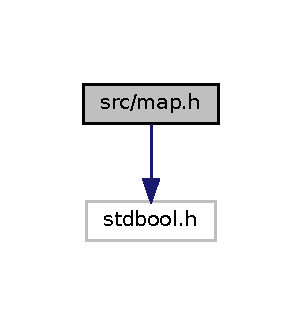
\includegraphics[width=145pt]{map_8h__incl}
\end{center}
\end{figure}
\subsection*{Typedefs}
\begin{DoxyCompactItemize}
\item 
typedef struct \hyperlink{map_8h_a767ff9e0c58d27b070f30636b66d2603}{Map} \hyperlink{map_8h_a767ff9e0c58d27b070f30636b66d2603}{Map}
\end{DoxyCompactItemize}
\subsection*{Functions}
\begin{DoxyCompactItemize}
\item 
\hyperlink{map_8h_a767ff9e0c58d27b070f30636b66d2603}{Map} $\ast$ \hyperlink{map_8h_ac192944f0151aabbf7a37a60d8eb7544}{new\+Map} (void)
\begin{DoxyCompactList}\small\item\em Tworzy nową strukturę. Tworzy nową, pustą strukturę niezawierającą żadnych miast, odcinków dróg ani dróg krajowych. \end{DoxyCompactList}\item 
void \hyperlink{map_8h_af9a88755f0e56e50088c87ce1f89c58f}{delete\+Map} (\hyperlink{map_8h_a767ff9e0c58d27b070f30636b66d2603}{Map} $\ast$map)
\begin{DoxyCompactList}\small\item\em Usuwa strukturę. Usuwa strukturę wskazywaną przez {\ttfamily map}. Nic nie robi, jeśli wskaźnik ten ma wartość N\+U\+LL. \end{DoxyCompactList}\item 
bool \hyperlink{map_8h_a51ef721938ddb094126ef3fa85f71446}{add\+Road} (\hyperlink{map_8h_a767ff9e0c58d27b070f30636b66d2603}{Map} $\ast$map, const char $\ast$city1, const char $\ast$city2, unsigned length, int built\+Year)
\begin{DoxyCompactList}\small\item\em Dodaje do mapy odcinek drogi między dwoma różnymi miastami. Jeśli któreś z podanych miast nie istnieje, to dodaje go do mapy, a następnie dodaje do mapy odcinek drogi między tymi miastami. \end{DoxyCompactList}\item 
bool \hyperlink{map_8h_ac0b4a4617c41f5b5438388f7273b0338}{repair\+Road} (\hyperlink{map_8h_a767ff9e0c58d27b070f30636b66d2603}{Map} $\ast$map, const char $\ast$city1, const char $\ast$city2, int repair\+Year)
\begin{DoxyCompactList}\small\item\em Modyfikuje rok ostatniego remontu odcinka drogi. Dla odcinka drogi między dwoma miastami zmienia rok jego ostatniego remontu lub ustawia ten rok, jeśli odcinek nie był jeszcze remontowany. \end{DoxyCompactList}\item 
bool \hyperlink{map_8h_ad3784ec559f14227533293e8ab67cec4}{new\+Route} (\hyperlink{map_8h_a767ff9e0c58d27b070f30636b66d2603}{Map} $\ast$map, unsigned route\+Id, const char $\ast$city1, const char $\ast$city2)
\begin{DoxyCompactList}\small\item\em Łączy dwa różne miasta drogą krajową. Tworzy drogę krajową pomiędzy dwoma miastami i nadaje jej podany numer. Wśród istniejących odcinków dróg wyszukuje najkrótszą drogę. Jeśli jest więcej niż jeden sposób takiego wyboru, to dla każdego wariantu wyznacza wśród wybranych w nim odcinków dróg ten, który był najdawniej wybudowany lub remontowany i wybiera wariant z odcinkiem, który jest najmłodszy. \end{DoxyCompactList}\item 
bool \hyperlink{map_8h_aa777e32bbe51fd78040b43ded577ec13}{extend\+Route} (\hyperlink{map_8h_a767ff9e0c58d27b070f30636b66d2603}{Map} $\ast$map, unsigned route\+Id, const char $\ast$city)
\begin{DoxyCompactList}\small\item\em Wydłuża drogę krajową do podanego miasta. Dodaje do drogi krajowej nowe odcinki dróg do podanego miasta w taki sposób, aby nowy fragment drogi krajowej był najkrótszy. Jeśli jest więcej niż jeden sposób takiego wydłużenia, to dla każdego wariantu wyznacza wśród dodawanych odcinków dróg ten, który był najdawniej wybudowany lub remontowany i wybiera wariant z odcinkiem, który jest najmłodszy. \end{DoxyCompactList}\item 
bool \hyperlink{map_8h_a9c60ffe680e512231cda53ff63cc5e76}{remove\+Road} (\hyperlink{map_8h_a767ff9e0c58d27b070f30636b66d2603}{Map} $\ast$map, const char $\ast$city1, const char $\ast$city2)
\begin{DoxyCompactList}\small\item\em Usuwa odcinek drogi między dwoma różnymi miastami. Usuwa odcinek drogi między dwoma miastami. Jeśli usunięcie tego odcinka drogi powoduje przerwanie ciągu jakiejś drogi krajowej, to uzupełnia ją istniejącymi odcinkami dróg w taki sposób, aby była najkrótsza. Jeśli jest więcej niż jeden sposób takiego uzupełnienia, to dla każdego wariantu wyznacza wśród dodawanych odcinków drogi ten, który był najdawniej wybudowany lub remontowany i wybiera wariant z odcinkiem, który jest najmłodszy. \end{DoxyCompactList}\item 
char const  $\ast$ \hyperlink{map_8h_aac086d65d78b4f834f79149bd4fdb95c}{get\+Route\+Description} (\hyperlink{map_8h_a767ff9e0c58d27b070f30636b66d2603}{Map} $\ast$map, unsigned route\+Id)
\begin{DoxyCompactList}\small\item\em Udostępnia informacje o drodze krajowej. Zwraca wskaźnik na napis, który zawiera informacje o drodze krajowej. Alokuje pamięć na ten napis. Zwraca pusty napis, jeśli nie istnieje droga krajowa o podanym numerze. Zaalokowaną pamięć trzeba zwolnić za pomocą funkcji free. Informacje wypisywane są w formacie\+: numer drogi krajowej;nazwa miasta;długość odcinka drogi;rok budowy lub ostatniego remontu;nazwa miasta;długość odcinka drogi;rok budowy lub ostatniego remontu;nazwa miasta;…;nazwa miasta. Kolejność miast na liście jest taka, aby miasta {\ttfamily city1} i {\ttfamily city2}, podane w wywołaniu funkcji \hyperlink{map_8h_ad3784ec559f14227533293e8ab67cec4}{new\+Route}, które utworzyło tę drogę krajową, zostały wypisane w tej kolejności. \end{DoxyCompactList}\end{DoxyCompactItemize}


\subsection{Detailed Description}
Interfejs klasy przechowującej mapę dróg krajowych

\begin{DoxyAuthor}{Author}
Łukasz Kamiński \href{mailto:kamis@mimuw.edu.pl}{\tt kamis@mimuw.\+edu.\+pl}, Marcin Peczarski \href{mailto:marpe@mimuw.edu.pl}{\tt marpe@mimuw.\+edu.\+pl} 
\end{DoxyAuthor}
\begin{DoxyCopyright}{Copyright}
Uniwersytet Warszawski 
\end{DoxyCopyright}
\begin{DoxyDate}{Date}
20.\+03.\+2019 
\end{DoxyDate}


\subsection{Typedef Documentation}
\mbox{\Hypertarget{map_8h_a767ff9e0c58d27b070f30636b66d2603}\label{map_8h_a767ff9e0c58d27b070f30636b66d2603}} 
\index{map.\+h@{map.\+h}!Map@{Map}}
\index{Map@{Map}!map.\+h@{map.\+h}}
\subsubsection{\texorpdfstring{Map}{Map}}
{\footnotesize\ttfamily typedef struct \hyperlink{map_8h_a767ff9e0c58d27b070f30636b66d2603}{Map} \hyperlink{map_8h_a767ff9e0c58d27b070f30636b66d2603}{Map}}

Struktura przechowująca mapę dróg krajowych. 

\subsection{Function Documentation}
\mbox{\Hypertarget{map_8h_a51ef721938ddb094126ef3fa85f71446}\label{map_8h_a51ef721938ddb094126ef3fa85f71446}} 
\index{map.\+h@{map.\+h}!add\+Road@{add\+Road}}
\index{add\+Road@{add\+Road}!map.\+h@{map.\+h}}
\subsubsection{\texorpdfstring{add\+Road()}{addRoad()}}
{\footnotesize\ttfamily bool add\+Road (\begin{DoxyParamCaption}\item[{\hyperlink{map_8h_a767ff9e0c58d27b070f30636b66d2603}{Map} $\ast$}]{map,  }\item[{const char $\ast$}]{city1,  }\item[{const char $\ast$}]{city2,  }\item[{unsigned}]{length,  }\item[{int}]{built\+Year }\end{DoxyParamCaption})}



Dodaje do mapy odcinek drogi między dwoma różnymi miastami. Jeśli któreś z podanych miast nie istnieje, to dodaje go do mapy, a następnie dodaje do mapy odcinek drogi między tymi miastami. 


\begin{DoxyParams}[1]{Parameters}
\mbox{\tt in,out}  & {\em map} & – wskaźnik na strukturę przechowującą mapę dróg; \\
\hline
\mbox{\tt in}  & {\em city1} & – wskaźnik na napis reprezentujący nazwę miasta; \\
\hline
\mbox{\tt in}  & {\em city2} & – wskaźnik na napis reprezentujący nazwę miasta; \\
\hline
\mbox{\tt in}  & {\em length} & – długość w km odcinka drogi; \\
\hline
\mbox{\tt in}  & {\em built\+Year} & – rok budowy odcinka drogi. \\
\hline
\end{DoxyParams}
\begin{DoxyReturn}{Returns}
Wartość {\ttfamily true}, jeśli odcinek drogi został dodany. Wartość {\ttfamily false}, jeśli wystąpił błąd\+: któryś z parametrów ma niepoprawną wartość, obie podane nazwy miast są identyczne, odcinek drogi między tymi miastami już istnieje lub nie udało się zaalokować pamięci. 
\end{DoxyReturn}
\mbox{\Hypertarget{map_8h_af9a88755f0e56e50088c87ce1f89c58f}\label{map_8h_af9a88755f0e56e50088c87ce1f89c58f}} 
\index{map.\+h@{map.\+h}!delete\+Map@{delete\+Map}}
\index{delete\+Map@{delete\+Map}!map.\+h@{map.\+h}}
\subsubsection{\texorpdfstring{delete\+Map()}{deleteMap()}}
{\footnotesize\ttfamily void delete\+Map (\begin{DoxyParamCaption}\item[{\hyperlink{map_8h_a767ff9e0c58d27b070f30636b66d2603}{Map} $\ast$}]{map }\end{DoxyParamCaption})}



Usuwa strukturę. Usuwa strukturę wskazywaną przez {\ttfamily map}. Nic nie robi, jeśli wskaźnik ten ma wartość N\+U\+LL. 


\begin{DoxyParams}[1]{Parameters}
\mbox{\tt in}  & {\em map} & – wskaźnik na usuwaną strukturę. \\
\hline
\end{DoxyParams}
\mbox{\Hypertarget{map_8h_aa777e32bbe51fd78040b43ded577ec13}\label{map_8h_aa777e32bbe51fd78040b43ded577ec13}} 
\index{map.\+h@{map.\+h}!extend\+Route@{extend\+Route}}
\index{extend\+Route@{extend\+Route}!map.\+h@{map.\+h}}
\subsubsection{\texorpdfstring{extend\+Route()}{extendRoute()}}
{\footnotesize\ttfamily bool extend\+Route (\begin{DoxyParamCaption}\item[{\hyperlink{map_8h_a767ff9e0c58d27b070f30636b66d2603}{Map} $\ast$}]{map,  }\item[{unsigned}]{route\+Id,  }\item[{const char $\ast$}]{city }\end{DoxyParamCaption})}



Wydłuża drogę krajową do podanego miasta. Dodaje do drogi krajowej nowe odcinki dróg do podanego miasta w taki sposób, aby nowy fragment drogi krajowej był najkrótszy. Jeśli jest więcej niż jeden sposób takiego wydłużenia, to dla każdego wariantu wyznacza wśród dodawanych odcinków dróg ten, który był najdawniej wybudowany lub remontowany i wybiera wariant z odcinkiem, który jest najmłodszy. 


\begin{DoxyParams}[1]{Parameters}
\mbox{\tt in,out}  & {\em map} & – wskaźnik na strukturę przechowującą mapę dróg; \\
\hline
\mbox{\tt in}  & {\em route\+Id} & – numer drogi krajowej; \\
\hline
\mbox{\tt in}  & {\em city} & – wskaźnik na napis reprezentujący nazwę miasta. \\
\hline
\end{DoxyParams}
\begin{DoxyReturn}{Returns}
Wartość {\ttfamily true}, jeśli droga krajowa została wydłużona. Wartość {\ttfamily false}, jeśli wystąpił błąd\+: któryś z parametrów ma niepoprawną nazwę, nie istnieje droga krajowa o podanym numerze, nie ma miasta o podanej nazwie, przez podane miasto już przechodzi droga krajowa o podanym numerze, podana droga krajowa kończy się w podanym mieście, nie można jednoznacznie wyznaczyć nowego fragmentu drogi krajowej lub nie udało się zaalokować pamięci. 
\end{DoxyReturn}
\mbox{\Hypertarget{map_8h_aac086d65d78b4f834f79149bd4fdb95c}\label{map_8h_aac086d65d78b4f834f79149bd4fdb95c}} 
\index{map.\+h@{map.\+h}!get\+Route\+Description@{get\+Route\+Description}}
\index{get\+Route\+Description@{get\+Route\+Description}!map.\+h@{map.\+h}}
\subsubsection{\texorpdfstring{get\+Route\+Description()}{getRouteDescription()}}
{\footnotesize\ttfamily char const$\ast$ get\+Route\+Description (\begin{DoxyParamCaption}\item[{\hyperlink{map_8h_a767ff9e0c58d27b070f30636b66d2603}{Map} $\ast$}]{map,  }\item[{unsigned}]{route\+Id }\end{DoxyParamCaption})}



Udostępnia informacje o drodze krajowej. Zwraca wskaźnik na napis, który zawiera informacje o drodze krajowej. Alokuje pamięć na ten napis. Zwraca pusty napis, jeśli nie istnieje droga krajowa o podanym numerze. Zaalokowaną pamięć trzeba zwolnić za pomocą funkcji free. Informacje wypisywane są w formacie\+: numer drogi krajowej;nazwa miasta;długość odcinka drogi;rok budowy lub ostatniego remontu;nazwa miasta;długość odcinka drogi;rok budowy lub ostatniego remontu;nazwa miasta;…;nazwa miasta. Kolejność miast na liście jest taka, aby miasta {\ttfamily city1} i {\ttfamily city2}, podane w wywołaniu funkcji \hyperlink{map_8h_ad3784ec559f14227533293e8ab67cec4}{new\+Route}, które utworzyło tę drogę krajową, zostały wypisane w tej kolejności. 


\begin{DoxyParams}[1]{Parameters}
\mbox{\tt in,out}  & {\em map} & – wskaźnik na strukturę przechowującą mapę dróg; \\
\hline
\mbox{\tt in}  & {\em route\+Id} & – numer drogi krajowej. \\
\hline
\end{DoxyParams}
\begin{DoxyReturn}{Returns}
Wskaźnik na napis lub N\+U\+LL, gdy nie udało się zaalokować pamięci. 
\end{DoxyReturn}
\mbox{\Hypertarget{map_8h_ac192944f0151aabbf7a37a60d8eb7544}\label{map_8h_ac192944f0151aabbf7a37a60d8eb7544}} 
\index{map.\+h@{map.\+h}!new\+Map@{new\+Map}}
\index{new\+Map@{new\+Map}!map.\+h@{map.\+h}}
\subsubsection{\texorpdfstring{new\+Map()}{newMap()}}
{\footnotesize\ttfamily \hyperlink{map_8h_a767ff9e0c58d27b070f30636b66d2603}{Map}$\ast$ new\+Map (\begin{DoxyParamCaption}\item[{void}]{ }\end{DoxyParamCaption})}



Tworzy nową strukturę. Tworzy nową, pustą strukturę niezawierającą żadnych miast, odcinków dróg ani dróg krajowych. 

\begin{DoxyReturn}{Returns}
Wskaźnik na utworzoną strukturę lub N\+U\+LL, gdy nie udało się zaalokować pamięci. 
\end{DoxyReturn}
\mbox{\Hypertarget{map_8h_ad3784ec559f14227533293e8ab67cec4}\label{map_8h_ad3784ec559f14227533293e8ab67cec4}} 
\index{map.\+h@{map.\+h}!new\+Route@{new\+Route}}
\index{new\+Route@{new\+Route}!map.\+h@{map.\+h}}
\subsubsection{\texorpdfstring{new\+Route()}{newRoute()}}
{\footnotesize\ttfamily bool new\+Route (\begin{DoxyParamCaption}\item[{\hyperlink{map_8h_a767ff9e0c58d27b070f30636b66d2603}{Map} $\ast$}]{map,  }\item[{unsigned}]{route\+Id,  }\item[{const char $\ast$}]{city1,  }\item[{const char $\ast$}]{city2 }\end{DoxyParamCaption})}



Łączy dwa różne miasta drogą krajową. Tworzy drogę krajową pomiędzy dwoma miastami i nadaje jej podany numer. Wśród istniejących odcinków dróg wyszukuje najkrótszą drogę. Jeśli jest więcej niż jeden sposób takiego wyboru, to dla każdego wariantu wyznacza wśród wybranych w nim odcinków dróg ten, który był najdawniej wybudowany lub remontowany i wybiera wariant z odcinkiem, który jest najmłodszy. 


\begin{DoxyParams}[1]{Parameters}
\mbox{\tt in,out}  & {\em map} & – wskaźnik na strukturę przechowującą mapę dróg; \\
\hline
\mbox{\tt in}  & {\em route\+Id} & – numer drogi krajowej; \\
\hline
\mbox{\tt in}  & {\em city1} & – wskaźnik na napis reprezentujący nazwę miasta; \\
\hline
\mbox{\tt in}  & {\em city2} & – wskaźnik na napis reprezentujący nazwę miasta. \\
\hline
\end{DoxyParams}
\begin{DoxyReturn}{Returns}
Wartość {\ttfamily true}, jeśli droga krajowa została utworzona. Wartość {\ttfamily false}, jeśli wystąpił błąd\+: któryś z parametrów ma niepoprawną wartość, istnieje już droga krajowa o podanym numerze, któreś z podanych miast nie istnieje, obie podane nazwy miast są identyczne, nie można jednoznacznie wyznaczyć drogi krajowej między podanymi miastami lub nie udało się zaalokować pamięci. 
\end{DoxyReturn}
\mbox{\Hypertarget{map_8h_a9c60ffe680e512231cda53ff63cc5e76}\label{map_8h_a9c60ffe680e512231cda53ff63cc5e76}} 
\index{map.\+h@{map.\+h}!remove\+Road@{remove\+Road}}
\index{remove\+Road@{remove\+Road}!map.\+h@{map.\+h}}
\subsubsection{\texorpdfstring{remove\+Road()}{removeRoad()}}
{\footnotesize\ttfamily bool remove\+Road (\begin{DoxyParamCaption}\item[{\hyperlink{map_8h_a767ff9e0c58d27b070f30636b66d2603}{Map} $\ast$}]{map,  }\item[{const char $\ast$}]{city1,  }\item[{const char $\ast$}]{city2 }\end{DoxyParamCaption})}



Usuwa odcinek drogi między dwoma różnymi miastami. Usuwa odcinek drogi między dwoma miastami. Jeśli usunięcie tego odcinka drogi powoduje przerwanie ciągu jakiejś drogi krajowej, to uzupełnia ją istniejącymi odcinkami dróg w taki sposób, aby była najkrótsza. Jeśli jest więcej niż jeden sposób takiego uzupełnienia, to dla każdego wariantu wyznacza wśród dodawanych odcinków drogi ten, który był najdawniej wybudowany lub remontowany i wybiera wariant z odcinkiem, który jest najmłodszy. 


\begin{DoxyParams}[1]{Parameters}
\mbox{\tt in,out}  & {\em map} & – wskaźnik na strukturę przechowującą mapę dróg; \\
\hline
\mbox{\tt in}  & {\em city1} & – wskaźnik na napis reprezentujący nazwę miasta; \\
\hline
\mbox{\tt in}  & {\em city2} & – wskaźnik na napis reprezentujący nazwę miasta. \\
\hline
\end{DoxyParams}
\begin{DoxyReturn}{Returns}
Wartość {\ttfamily true}, jeśli odcinek drogi został usunięty. Wartość {\ttfamily false}, jeśli z powodu błędu nie można usunąć tego odcinka drogi\+: któryś z parametrów ma niepoprawną wartość, nie ma któregoś z podanych miast, nie istnieje droga między podanymi miastami, nie da się jednoznacznie uzupełnić przerwanego ciągu drogi krajowej lub nie udało się zaalokować pamięci. 
\end{DoxyReturn}
\mbox{\Hypertarget{map_8h_ac0b4a4617c41f5b5438388f7273b0338}\label{map_8h_ac0b4a4617c41f5b5438388f7273b0338}} 
\index{map.\+h@{map.\+h}!repair\+Road@{repair\+Road}}
\index{repair\+Road@{repair\+Road}!map.\+h@{map.\+h}}
\subsubsection{\texorpdfstring{repair\+Road()}{repairRoad()}}
{\footnotesize\ttfamily bool repair\+Road (\begin{DoxyParamCaption}\item[{\hyperlink{map_8h_a767ff9e0c58d27b070f30636b66d2603}{Map} $\ast$}]{map,  }\item[{const char $\ast$}]{city1,  }\item[{const char $\ast$}]{city2,  }\item[{int}]{repair\+Year }\end{DoxyParamCaption})}



Modyfikuje rok ostatniego remontu odcinka drogi. Dla odcinka drogi między dwoma miastami zmienia rok jego ostatniego remontu lub ustawia ten rok, jeśli odcinek nie był jeszcze remontowany. 


\begin{DoxyParams}[1]{Parameters}
\mbox{\tt in,out}  & {\em map} & – wskaźnik na strukturę przechowującą mapę dróg; \\
\hline
\mbox{\tt in}  & {\em city1} & – wskaźnik na napis reprezentujący nazwę miasta; \\
\hline
\mbox{\tt in}  & {\em city2} & – wskaźnik na napis reprezentujący nazwę miasta; \\
\hline
\mbox{\tt in}  & {\em repair\+Year} & – rok ostatniego remontu odcinka drogi. \\
\hline
\end{DoxyParams}
\begin{DoxyReturn}{Returns}
Wartość {\ttfamily true}, jeśli modyfikacja się powiodła. Wartość {\ttfamily false}, jeśli wystąpił błąd\+: któryś z parametrów ma niepoprawną wartość, któreś z podanych miast nie istnieje, nie ma odcinka drogi między podanymi miastami, podany rok jest wcześniejszy niż zapisany dla tego odcinka drogi rok budowy lub ostatniego remontu. 
\end{DoxyReturn}

%--- End generated contents ---

% Index
\backmatter
\newpage
\phantomsection
\clearemptydoublepage
\addcontentsline{toc}{chapter}{Index}
\printindex

\end{document}
